\chapter{Etat de l'art}

\section{problème de flow-shop avec permutation}
Le problème de flow-shop avec permutation est un problème où l'on cherche à trouver l'ordre dans lequel réaliser des jobs.
Dans ce problème, chaque job doit passer par différentes machines, toujours dans le même ordre.

Pour ce problème, les solutions sont généralement représentées sous la forme de diagramme de Gantt.

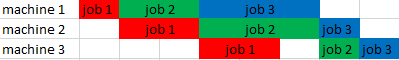
\includegraphics{parts/etat_de_l_art/gantt_exemple.png}

\section{problème de routing}
\section{Recherche locale}
\label{section:recherche_locale}

Les algorithmes de recherche locale permettent de chercher une bonne solution en apportant des améliorations successives à une solution.

A partir d'une solution, on explore les solutions voisines (qui sont obtenus en appliquant un opérateur de voisinage sur la solution).
Parmi ces solutions, on en prend une qui donne un meilleur score.

\begin{algorithm}
	\caption{Algorithme de recherche locale} 
	\label{algo:recherche_locale}
	\SetKwRepeat{Repeat}{répéter}{tant que}
	\SetKwIF{If}{ElseIf}{Else}{si}{alors}{sinon si}{sinon}{fin}
	\SetKwFor{ForEach}{pout toutes}{faire}{fin}

	\tcc{$solution\_actuelle$ : une solution générée aléatoirement}
	\tcc{$F(s)$ : la fonction objectif à minimiser}
	\tcc{$Operateur\_de\_voisinnage(s)$ : une fonction qui donne la liste des solutions voisines à la solution s.}
	$meilleure\_voisine \gets solution\_actuelle$

	\Repeat{$F(solution\_actuelle) < F(meilleure\_voisine)$ }
	{
		$solution\_actuelle \gets meilleure\_voisine$

		\ForEach{$solution\_voisine$ de $Operateur\_de\_voisinnage(solution\_actuelle)$}
		{
			\If{$F(solution\_voisine) < F(meilleure\_voisine)$}
			{
				$meilleure\_voisine \gets solution\_voisine$
			}
		}
	}
\end{algorithm}